\documentclass[tikz=true]{standalone}
\usepackage{amsmath}
\usepackage{amsfonts}
\usepackage{tikz}
\usepackage{relsize}
\usepackage{mathtools}
\usepackage{bm}

\definecolor{lightGreen}{rgb}{.56, .93, .56}
\definecolor{lightPink}{rgb}{1, .71, .76}
\definecolor{cornflowerBlue}{RGB}{100, 149, 237}
\definecolor{navajoWhite}{rgb}{1, 0.87, 0.68}
\definecolor{darkSeaGreen}{rgb}{.56, 0.74, 0.56}
\definecolor{purple}{rgb}{.63, .13, .94}
\definecolor{teal}{rgb}{0, .5, .5}
\DeclarePairedDelimiter\abs{\lvert}{\rvert}%
\newcommand{\vv}{\ensuremath{\,\vert\,}}
\newcommand{\cc}{\ensuremath{,\,}}
\newcommand{\expnumber}[2]{{#1}\mathrm{e}{#2}}
% Symbol declaration as macros

\newcommand{\pdel}{\ensuremath{p_D}}
\newcommand{\pins}{\ensuremath{p_I}}
\newcommand{\psub}{\ensuremath{p_S}}
\newcommand{\ptrans}{\ensuremath{p_T}}
\newcommand{\sbin}{\ensuremath{\{ 0, 1\}}}
\newcommand{\ibin}{\ensuremath{[ 0, 1]}}
% \newcommand{\sset}[1]{\ensuremath{\{ #1 \}}}

% generic codeword y 

\newcommand{\ygen}{\ensuremath{\bm{x}}}
\newcommand{\ygenIx}{\ensuremath{x}}


% inner encoded y 
\newcommand{\yin}{\ensuremath{\bm{x}^{\text{in}}}}
% outer encoded y 
\newcommand{\yout}{\ensuremath{\bm{x}^{\text{out}}}}

% inner encoded y _ ix => scalar
\newcommand{\yinIx}{\ensuremath{x^{\text{in}}}}


% outer encoded y _ix => scalar
\newcommand{\youtIx}{\ensuremath{x^{\text{out}}}}


\newcommand{\Yval}{\ensuremath{\xi}}
% message m 
\newcommand{\mess}{\ensuremath{\bm{m}}}

% mess Prediction
\newcommand{\messPred}{\ensuremath{\bm{\hat{m}}}}

% length fo a generic codeword
\newcommand{\ngen}{\ensuremath{n}}
% length of inner encoded y 
\newcommand{\nin}{\ensuremath{n_{\text{in}}}}

% length of outer encoded y 
\newcommand{\nout}{\ensuremath{n_{\text{out}}}}


% prediction of outer encoded y
\newcommand{\predyout}{\ensuremath{\bm{\hat{x}}^{\text{out}}}}
\newcommand{\predyin}{\ensuremath{\bm{\hat{x}}^{\text{in}}}}
% received sequence
\newcommand{\rec}{\ensuremath{\bm{r}}}

\newcommand{\recIx}{\ensuremath{r}}

% received sequence of a bpsk channel
\newcommand{\recbpsk}{\ensuremath{\bm{r}^{\text{BPSK}}}}

% length of a sequence received via the bpsk channel
\newcommand{\nrecbpsk}{\ensuremath{\nout}} 

% length of received sequence
\newcommand{\nrec}{\ensuremath{n_{\text{rec}}}}

\newcommand{\dfrom}{\ensuremath{d}}
\newcommand{\dto}{\ensuremath{d^{\prime}}}

\newcommand{\llin}{\ensuremath{\text{Lin}}}

\newcommand{\llr}{\ensuremath{\text{LLR}}}
\newcommand{\bipolar}{\ensuremath{\phi}}
\newcommand{\syndrome}{\ensuremath{\text{syn}}}
\newcommand{\bin}{\ensuremath{\text{bin}}}

\newcommand{\ybipolar}{\ensuremath{\bm{x}^{\bipolar}}}


\newcommand{\ymodel}{\ensuremath{\bm{\hat{x}}}}
\newcommand{\ymodelIx}{\ensuremath{\hat{x}}}

% \newcommand{\gftwo}{\ensuremath{\mathbb{F}_2}}

\newcommand{\marker}{\ensuremath{\bm{s_m}}}
\newcommand{\markerFreq}{\ensuremath{N_m}}


\newcommand{\gen}{\ensuremath{\bm{G}}}
\newcommand{\pc}{\ensuremath{\bm{H}}}
\newcommand{\attQuery}{\ensuremath{\bm{Q}}}
\newcommand{\attKey}{\ensuremath{\bm{K}}}
\newcommand{\attValue}{\ensuremath{\bm{V}}}

\newcommand{\alphabetSize}{\ensuremath{q}}

\newcommand{\bcjrformerInput}{\ensuremath{\bm{Y}}}
\newcommand{\bcjrformerInputIx}{\ensuremath{Y}}

\newcommand{\bcjrformerInputBit}{\ensuremath{\bm{Y^{\text{symb}}}}}
\newcommand{\bcjrformerInputBitIx}{\ensuremath{Y^{\text{symb}}}}

\newcommand{\bcjrformerInputState}{\ensuremath{\bm{Y^{\text{state}}}}}
\newcommand{\bcjrformerInputStateIx}{\ensuremath{Y^{\text{state}}}}

\newcommand{\alphabet}{\ensuremath{\mathbb{F}_q}}

\newcommand{\nstates}{\ensuremath{n_s}}

\newcommand{\offset}{\ensuremath{\bm{o}}}
\newcommand{\offsetIx}{\ensuremath{o}}

\tikzset{fontscale/.style = {font=\relsize{#1}}
    }


\usetikzlibrary {arrows, calc,positioning,shapes.misc, graphs, matrix, fit, quotes, backgrounds, decorations.pathreplacing}

\tikzstyle{layerNode} = [draw=black, line width=.5pt, rectangle, rounded corners = 2pt, minimum height = 10pt]

\tikzstyle{symbolReprNode} = [draw=black, rectangle, minimum height=12pt, minimum width=4pt, inner sep=0]

\tikzstyle{stateReprNode} = [draw=black, rectangle, minimum height=12pt, minimum width=8pt, inner sep=0]

\tikzstyle{outputReprNode} = [draw=black, rectangle, minimum height=4pt, minimum width=4pt, inner sep=0]

% \tikzstyle{addNode} = [draw=black, circle, inner sep=0]

\tikzstyle{addNode} = [
    circle,
    draw=black,
    inner sep=0,
    minimum size=7pt,
    path picture={
      \draw [black]
            (path picture bounding box.90) -- (path picture bounding box.270)
            (path picture bounding box.0) -- (path picture bounding box.180);
    }
]


\begin{document}

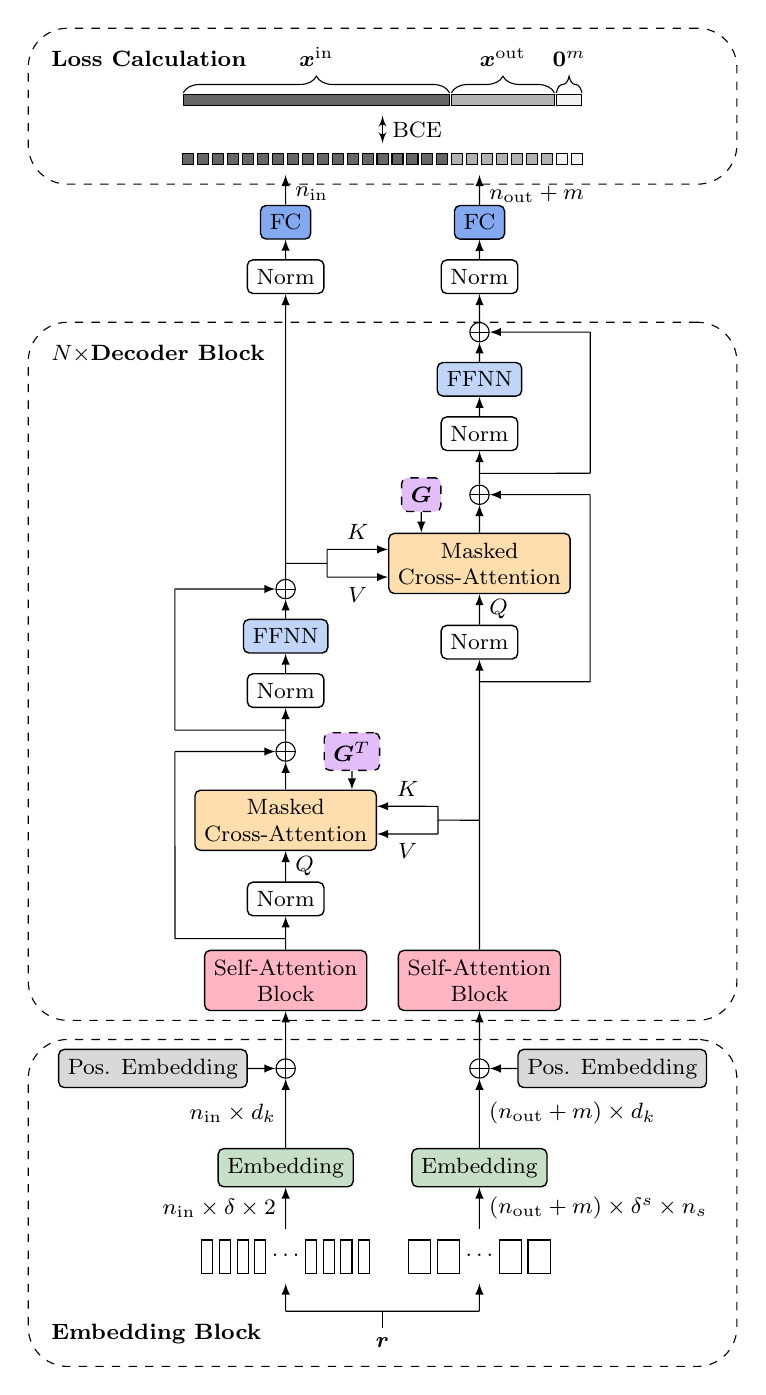
\begin{tikzpicture}[font=\footnotesize, scale=.1]       
% \node[vnode, right = 10pt of v3.east] (v4) {$v_4$};

% \draw[step=1.0,black, opacity=.2,thin] (-200pt, -50pt) grid (200pt,800pt);

\node(rec) at (0,0) {$\bm{r}$};

% Received Sequence to Input
\node[coordinate, above = 6pt of rec.north] (coordRecSplit){};
\node[coordinate, left = 35pt of coordRecSplit] (coordRecSplitLeft){};
\node[coordinate, right = 35pt of coordRecSplit] (coordRecSplitRight){};

% Input Creation
\matrix(symbolInput)[row sep=0pt,column sep=2pt, matrix of nodes, nodes={symbolReprNode}, nodes in empty cells, above = 10pt of coordRecSplitLeft] {
 & & & & |[draw=none]| $\ldots$& & & & \\
};
\matrix(stateInput)[row sep=0pt,column sep=2pt, matrix of nodes, nodes={stateReprNode}, nodes in empty cells, above = 10pt of coordRecSplitRight] {
 & &|[draw=none]| $\ldots$ & &  \\
};

% Linear Embeddings
\node (symbolLinEmb)[layerNode, fill=darkSeaGreen!50, above = 15pt of symbolInput] {Embedding};
\node (stateLinEmb)[layerNode, fill=darkSeaGreen!50, above = 15pt of stateInput] {Embedding};

% Positional Embedding
\node (symbolPosEmbAdd)[addNode, above = 25pt of symbolLinEmb] {};
\node (statePosEmbAdd)[addNode, above = 25pt of stateLinEmb] {};

\node(symbolPosEmb)[layerNode, fill=gray!30, left = 10pt of symbolPosEmbAdd] {Pos. Embedding};
\node(statePosEmb)[layerNode, fill=gray!30,right = 10pt of statePosEmbAdd] {Pos. Embedding};

% Self Attention / Transformer Layer

\node (symbolSelfAttention)[layerNode, fill=lightPink, above = 17pt of symbolPosEmbAdd, align=center] {Self-Attention \\ Block};
\node (stateSelfAttention)[layerNode, fill=lightPink, above = 17pt of statePosEmbAdd, align=center] {Self-Attention \\ Block};

% Cross Attention: Symbol => State
\node (symbolResidualStart)[coordinate, above=4pt of symbolSelfAttention] {};
\node (symbolResidualP1)[coordinate, left = 40pt of symbolResidualStart] {};

\node (symbolLayerNorm)[layerNode, above = 8pt of symbolResidualStart] {Norm};
\node (symbolLayerCrossAttn)[layerNode, fill=navajoWhite, above = 11pt of symbolLayerNorm, align = center] {Masked \\ Cross-Attention};

\node (symbolResidualAdd) [addNode, above =10pt of symbolLayerCrossAttn] {};
\node (symbolResidualP2)[coordinate, left=40pt of symbolResidualAdd.center] {};
\node (symbolGeneratorMask)[layerNode, dashed, fill=purple!30, right = 10pt of symbolResidualAdd, anchor=west] {$\gen^T$};
% intersection point for vertical line downwards from G into Cross Attention Layer
\node(symbolIntersectionGeneratorCrossAttn)[coordinate] at (symbolLayerCrossAttn.north -| symbolGeneratorMask) {};

% Self Attention (State) To Cross Attention
\node(symbolIntersectionCrossAttnState)[coordinate] at (symbolLayerCrossAttn.east -| stateSelfAttention) {};
\node(symbolKeyValueSplit)[coordinate, left = 15pt of symbolIntersectionCrossAttnState] {};

\node(symbolKeyPathStart)[coordinate, above = 5pt of symbolKeyValueSplit] {};
\node(symbolKeyPathEnd)[coordinate] at (symbolLayerCrossAttn.east |- symbolKeyPathStart) {};

\node(symbolValuePathStart)[coordinate, below = 5pt of symbolKeyValueSplit] {};
\node(symbolValuePathEnd)[coordinate] at (symbolLayerCrossAttn.east |- symbolValuePathStart) {};

\node (symbolResidual2Start)[coordinate, above=4pt of symbolResidualAdd] {};
\node (symbolResidual2P1)[coordinate, left = 40pt of symbolResidual2Start] {};
\node (symbolLayerNorm2)[layerNode, above = 8pt of symbolResidual2Start] {Norm};
\node (symbolFeedForwardLayer)[layerNode, fill= cornflowerBlue!40, above= 7pt of symbolLayerNorm2] {FFNN};

\node (symbolResidual2Add) [addNode, above =7pt of symbolFeedForwardLayer] {};
\node (symbolResidual2P2)[coordinate, left=40pt of symbolResidual2Add.center] {};


% Cross Attention: State => Symbol
\node (stateResidualStart)[coordinate, above=50pt of symbolIntersectionCrossAttnState] {};
\node (stateResidualP1)[coordinate, right = 40pt of stateResidualStart] {};

\node (stateLayerNorm)[layerNode, above = 8pt of stateResidualStart] {Norm};
\node (stateLayerCrossAttn)[layerNode, fill=navajoWhite, above = 11pt of stateLayerNorm, align = center] {Masked \\ Cross-Attention};

\node (stateResidualAdd) [addNode, above =10pt of stateLayerCrossAttn] {};
\node (stateResidualP2)[coordinate, right=40pt of stateResidualAdd.center] {};
\node (stateGeneratorMask)[layerNode, dashed, fill=purple!30, left = 10pt of stateResidualAdd, anchor=east] {$\gen$};
% intersection point for vertical line downwards from G into Cross Attention Layer
\node(stateIntersectionGeneratorCrossAttn)[coordinate] at (stateLayerCrossAttn.north -| stateGeneratorMask) {};

% Layer (Symbol) To Cross Attention
\node(stateIntersectionCrossAttnSymbol)[coordinate] at (stateLayerCrossAttn.west -| symbolResidual2Add) {};
\node(stateKeyValueSplit)[coordinate, right = 15pt of stateIntersectionCrossAttnSymbol] {};

\node(stateKeyPathStart)[coordinate, above = 5pt of stateKeyValueSplit] {};
\node(stateKeyPathEnd)[coordinate] at (stateLayerCrossAttn.west |- stateKeyPathStart) {};

\node(stateValuePathStart)[coordinate, below = 5pt of stateKeyValueSplit] {};
\node(stateValuePathEnd)[coordinate] at (stateLayerCrossAttn.west |- stateValuePathStart) {};

\node (stateResidual2Start)[coordinate, above=4pt of stateResidualAdd] {};
\node (stateResidual2P1)[coordinate, right = 40pt of stateResidual2Start] {};
\node (stateLayerNorm2)[layerNode, above = 8pt of stateResidual2Start] {Norm};
\node (stateFeedForwardLayer)[layerNode, fill= cornflowerBlue!40, above= 7pt of stateLayerNorm2] {FFNN};

\node (stateResidual2Add) [addNode, above =7pt of stateFeedForwardLayer] {};
\node (stateResidual2P2)[coordinate, right=40pt of stateResidual2Add.center] {};

% Combination of both paths

\node (symbolOut)[coordinate] at (stateIntersectionCrossAttnSymbol |- stateResidual2Add.north) {};



% Feed Forward Head into Output Logits
\node (symbolLayerNormHead)[layerNode, above=10pt of symbolOut] {Norm};
\node (symbolFeedForwardHead)[layerNode, fill=cornflowerBlue!80, above=7pt of symbolLayerNormHead] {FC};

\node (stateLayerNormHead)[layerNode, above=10pt of stateResidual2Add.north] {Norm};
\node (stateFeedForwardHead)[layerNode, fill=cornflowerBlue!80, above=7pt of stateLayerNormHead] {FC};

\node[coordinate] (fullOutputAlignment) at ($(stateFeedForwardHead)!0.5!(symbolFeedForwardHead)$) {};

\matrix(fullOutput)[row sep=0pt,column sep=1pt, matrix of nodes, nodes={outputReprNode, fill=black!60}, nodes in empty cells, above = 17pt of fullOutputAlignment] {
 & & & & & & & & & & & & & & &  & & & |[fill=gray!60]|  & |[fill=gray!60]|  & |[fill=gray!60]| & |[fill=gray!60]| & |[fill=gray!60]| & |[fill=gray!60]| & |[fill=gray!60]| & |[fill=gray!10]| & |[fill=gray!10]| \\
};

\node (symbolFullOutputIntersection)[coordinate] at (symbolLayerNormHead |- fullOutput.south) {};
\node (stateFullOutputIntersection)[coordinate] at (stateLayerNormHead |- fullOutput.south) {};

\matrix(lossIllustration)[row sep=0pt,column sep=.5pt, matrix of nodes, nodes={outputReprNode}, nodes in empty cells, above = 10pt of fullOutput] {
 |[minimum width=96pt, fill=black!60](yIn)| & |[minimum width=37, fill=gray!60](yOut)| & |[minimum width=9, fill=gray!10] (memory)|\\
};





%%%% PATHS %%%% 

% Received Sequence to Input
\path (rec) edge[-] (coordRecSplit);
\path (coordRecSplit) edge[-] (coordRecSplitLeft);
\path (coordRecSplit) edge[-] (coordRecSplitRight);

% Input Creation
\path (coordRecSplitRight) edge[-latex] (stateInput);
\path (coordRecSplitLeft) edge[-latex] (symbolInput);

% Linear Embeddings
\path (symbolInput) edge[-latex] node[left] {$\nin \times \delta \times 2$} (symbolLinEmb);
\path (stateInput) edge[-latex] node[right] {$(\nout + m) \times \delta^s \times n_s$} (stateLinEmb);

% Positional Embedding
\path (symbolLinEmb) edge[-latex] node[left] {$\nin \times d_k$} (symbolPosEmbAdd);
\path (stateLinEmb) edge[-latex] node[right] {$(\nout + m) \times d_k$} (statePosEmbAdd);
\path (symbolPosEmb) edge[-latex] (symbolPosEmbAdd);
\path (statePosEmb) edge[-latex] (statePosEmbAdd);

% Self Attention
\path (symbolPosEmbAdd) edge[-latex] (symbolSelfAttention);
\path (statePosEmbAdd) edge[-latex] (stateSelfAttention);


%%% Cross Attention (Symbol => State)

% Cross Attention (Main)
\path (symbolResidualStart) edge[-latex] (symbolLayerNorm);
\path (symbolLayerNorm) edge[-latex] node[right] {$Q$}(symbolLayerCrossAttn);
\path (symbolLayerCrossAttn) edge[-latex] (symbolResidualAdd);

\path (symbolGeneratorMask) edge[-latex] (symbolIntersectionGeneratorCrossAttn);

% Residual Connection (Cross Attention)
\path (symbolSelfAttention) edge[-] (symbolResidualStart);
\path (symbolResidualStart) edge[-] (symbolResidualP1);
\path (symbolResidualP1) edge[-] (symbolResidualP2);
\path (symbolResidualP2) edge[-latex] (symbolResidualAdd);

% Key Value (From State Head)
\path (stateSelfAttention) edge[-] (symbolIntersectionCrossAttnState);

\path (symbolIntersectionCrossAttnState) edge[-] (symbolKeyValueSplit);
\path (symbolKeyValueSplit) edge[-] (symbolKeyPathStart);
\path (symbolKeyPathStart) edge[-latex] node[above] {$K$}(symbolKeyPathEnd);
\path (symbolKeyValueSplit) edge[-] (symbolValuePathStart);
\path (symbolValuePathStart) edge[-latex]  node[below] {$V$}(symbolValuePathEnd);

%%% Feed Forward Block (Symbol)
\path (symbolResidual2Start) edge[-latex] (symbolLayerNorm2);
\path (symbolLayerNorm2) edge[-latex] (symbolFeedForwardLayer);
\path (symbolFeedForwardLayer) edge[-latex] (symbolResidual2Add);

% Residual Connection
\path (symbolResidualAdd) edge[-] (symbolResidual2Start);
\path (symbolResidual2Start) edge[-] (symbolResidual2P1);
\path (symbolResidual2P1) edge[-] (symbolResidual2P2);
\path (symbolResidual2P2) edge[-latex] (symbolResidual2Add);


%%% Cross Attention (State => Symbol)

% Cross Attention (Main)
\path (stateResidualStart) edge[-latex] (stateLayerNorm);
\path (stateLayerNorm) edge[-latex] node[right] {$Q$}(stateLayerCrossAttn);
\path (stateLayerCrossAttn) edge[-latex] (stateResidualAdd);

\path (stateGeneratorMask) edge[-latex] (stateIntersectionGeneratorCrossAttn);

% Residual Connection (Cross Attention)
\path (symbolIntersectionCrossAttnState) edge[-] (stateResidualStart);
\path (stateResidualStart) edge[-] (stateResidualP1);
\path (stateResidualP1) edge[-] (stateResidualP2);
\path (stateResidualP2) edge[-latex] (stateResidualAdd);

% Key Value (From Symbol Head)
\path (symbolResidual2Add) edge[-] (stateIntersectionCrossAttnSymbol);

\path (stateIntersectionCrossAttnSymbol) edge[-] (stateKeyValueSplit);
\path (stateKeyValueSplit) edge[-] (stateKeyPathStart);
\path (stateKeyPathStart) edge[-latex] node[above] {$K$}(stateKeyPathEnd);
\path (stateKeyValueSplit) edge[-] (stateValuePathStart);
\path (stateValuePathStart) edge[-latex]  node[below] {$V$}(stateValuePathEnd);

%%% Feed Forward Block (Symbol)
\path (stateResidual2Start) edge[-latex] (stateLayerNorm2);
\path (stateLayerNorm2) edge[-latex] (stateFeedForwardLayer);
\path (stateFeedForwardLayer) edge[-latex] (stateResidual2Add);

% Residual Connection
\path (stateResidualAdd) edge[-] (stateResidual2Start);
\path (stateResidual2Start) edge[-] (stateResidual2P1);
\path (stateResidual2P1) edge[-] (stateResidual2P2);
\path (stateResidual2P2) edge[-latex] (stateResidual2Add);

%%% Output Layer

% from state
% \path (stateResidual2Add) edge [-] (stateOut);
\path (stateResidual2Add) edge [-latex] (stateLayerNormHead);
% from symbol
% \path (stateIntersectionCrossAttnSymbol) edge [-] (symbolOut);
\path (stateIntersectionCrossAttnSymbol) edge[-latex] (symbolLayerNormHead);

%%% MLP Head
\path (symbolLayerNormHead) edge [-latex] (symbolFeedForwardHead);
\path (stateLayerNormHead) edge [-latex] (stateFeedForwardHead);

% \path (symbolLayerNormHead) edge [-latex]node[right, yshift=-1.5pt] {$\nin$}  (symbolFeedForwardHead);

%%% Loss Calculation
\path (symbolFeedForwardHead) edge [-latex] node[right, yshift=-1.5pt] {$\nin$} (symbolFullOutputIntersection);
\path (stateFeedForwardHead) edge [-latex] node[right, yshift=-1.5pt] {$\nout + m$} (stateFullOutputIntersection);

\path (fullOutput) edge [latex'-latex'] node[right] {$\text{BCE}$} (lossIllustration);

\path[draw,decorate,decoration={brace, amplitude=6pt}] ([yshift=3pt, xshift=1pt]yIn.north west) -- ([yshift=3pt, xshift=-1pt]yIn.north east) node[midway,above, yshift=6pt,](yInLabel){$\yin$};
\path[draw,decorate,decoration={brace, amplitude=6pt}] ([yshift=3pt, xshift=1pt]yOut.north west) -- ([yshift=3pt, xshift=-1pt]yOut.north east) node[midway,above, yshift=6pt,]{$\yout$};
\path[draw,decorate,decoration={brace, amplitude=6pt}] ([yshift=3pt, xshift=1pt]memory.north west) -- ([yshift=3pt, xshift=-1pt]memory.north east) node[midway,above, yshift=6pt,]{$\bm{0}^m$};

%%% 

%%%% Containers
\begin{pgfonlayer}{background}
% Container for Embedding Block
\node (ContainerEmbedding) [rectangle, rounded corners= 5mm,  dashed, draw, minimum width=9cm, fit=(symbolPosEmb) (statePosEmb) (rec), label={[shift={(5pt,5pt)}, anchor=south west]south west:\textbf{Embedding Block}}] {};

% Container for One Decoder Layer

% Helper Coordinate to place top border of container a bit more north/south
\node[coordinate] (stateResidual2AddMoreNorth) at ([yshift=2pt]stateResidual2Add.center) {};

\node (ContainerDecoderLayer) [rectangle, rounded corners= 5mm, dashed, draw, minimum width=9cm, fit=(stateResidual2AddMoreNorth) (symbolSelfAttention) (stateResidual2P1) (symbolResidual2P1), label={[shift={(5pt,-5pt)}, anchor=north west]north west:$N\times$\textbf{Decoder Block}}] {};



% Container for the Loss "Layer"
\node (ContainerLossLayer) [rectangle, rounded corners= 5mm, dashed, draw, minimum width=9cm, fit=(fullOutput) (lossIllustration) (yInLabel), label={[shift={(5pt,-5pt)}, anchor=north west]north west:\textbf{Loss Calculation}}] {};

\end{pgfonlayer}


\end{tikzpicture}
\end{document}